\documentclass[letterpaper,10pt]{article}

\usepackage{titling}
\usepackage{listings}
\usepackage{url}
\usepackage{setspace}
\usepackage{subfig}
\usepackage{sectsty}
\usepackage{pdfpages}
\usepackage{colortbl}
\usepackage{multirow}
\usepackage{relsize}
\usepackage{amsmath}
\usepackage{fancyvrb}
\usepackage{amsmath,amssymb,amsthm,graphicx,xspace}
\usepackage[titlenotnumbered,noend,noline]{algorithm2e}
\usepackage[compact]{titlesec}
\usepackage[default]{droidserif}
\usepackage[T1]{fontenc}
\usepackage{tikz}
\usetikzlibrary{arrows,automata,shapes,trees,matrix,chains,scopes,positioning,calc}
\tikzstyle{block} = [rectangle, draw, fill=blue!20, 
    text width=2.5em, text centered, rounded corners, minimum height=2em]
\tikzstyle{bw} = [rectangle, draw, fill=blue!20, 
    text width=4em, text centered, rounded corners, minimum height=2em]

\definecolor{namerow}{cmyk}{.40,.40,.40,.40}
\definecolor{namecol}{cmyk}{.40,.40,.40,.40}

\let\LaTeXtitle\title
\renewcommand{\title}[1]{\LaTeXtitle{\textsf{#1}}}


\newcommand{\handout}[5]{
  \noindent
  \begin{center}
  \framebox{
    \vbox{
      \hbox to 5.78in { {\bf ECE155: Engineering Design with Embedded Systems } \hfill #2 }
      \vspace{4mm}
      \hbox to 5.78in { {\Large \hfill #4  \hfill} }
      \vspace{2mm}
      \hbox to 5.78in { {\em #3 \hfill} }
    }
  }
  \end{center}
  \vspace*{4mm}
}

\newcommand{\lecture}[3]{\handout{#1}{#2}{#3}{Lecture #1}}
\newcommand{\tuple}[1]{\ensuremath{\left\langle #1 \right\rangle}\xspace}

\addtolength{\oddsidemargin}{-1.000in}
\addtolength{\evensidemargin}{-0.500in}
\addtolength{\textwidth}{2.0in}
\addtolength{\topmargin}{-1.000in}
\addtolength{\textheight}{1.75in}
\addtolength{\parskip}{\baselineskip}
\setlength{\parindent}{0in}
\renewcommand{\baselinestretch}{1.5}
\newcommand{\term}{Spring 2014}

\singlespace


\begin{document}

\lecture{ 27 --- Verification \& Validation; SW Maintenance}{\term}{Patrick Lam \& Jeff Zarnett}

\section*{Verification and Validation}
It's important to not confuse the two related topics of verification
and validation. In \emph{verification}, we assume a set of
requirements and establish that the product satisfies the
requirements. The requirements might be wrong, but we can put up a
``Someone Else's Problem'' field and say that it's not our problem
when doing verification. \emph{Validation} is making sure that the
requirements are the right ones.

\paragraph{Verification.} We've already seen one form of verification:
\emph{testing}. The other option is \emph{static analysis}, which amounts
to having computers pore over the code or design. (``Building the thing right.'')

\paragraph{Validation.} Validation ensures that a project fully satisfies 
the needs of its customers. (How does XP incorporate validation?)
Validation should therefore go beyond checking that code meets
specifications and work with the customer to ensure that the
specifications are correct. (``Building the right thing.'')

One way to validate code is through \emph{beta testing}: customers
try out early versions of the software and determine whether or not 
it is doing the right thing.

Validation usually follows verification. It's not productive to
validate buggy software, but taking too long in verification can
result in validating high-quality code that satisfies the wrong
specification.

\paragraph{Recap.} The terms are similar, but:
\begin{itemize}
\item Verification answers the question, ``Is the project being built correctly?''
\item Validation answer the question, ``Will the project meet the needs of its users?''
\end{itemize}

You need to verify \emph{and} validate; projects can fail because they're
properly-built but don't meet needs; or they can sort-of meet users' needs
except that they don't work right.

In some cases, the verification and validation processes are carried out by a different team than developed the software. This is known as independent verification and validation. It is common in cases where there is extreme expense or risk to human life or health. NASA, for example, established independent verification and validation in 1993 to ensure the highest possible level of safety for mission-critical software. 

Validation might be required given a regulatory environment. The US Food and Drug Administration (FDA) requires software patches to be validated for networked medical devices. The device manufacturer bears responsibility for the safe and effective performance of the device, and the FDA will review when a change or modification could significantly affect the safety or effectiveness of the device~\cite{fda}. 

A successful project must pass both verification and validation.


\section*{Formal Methods}
Formal methods includes a variety of techniques for verifying that
code or designs conforms to a specification. Static analysis is a
formal methods technique, usually at code, or implementation,
level. It's possible to formally verify system designs as well as
implementations.

\paragraph{Key Idea.} To use formal methods, you need a model of the
artifact in question, along with a property that you would like to
verify. The model is often some sort of abstract graph representing
system behaviours, while the property is usually some sort of
(temporal logic) formula. Verification exhaustively
searches the model for violations of the property; it either tells
you that the property holds, or it shows you a counterexample.
By being clever, it's possible to verify huge state spaces
(e.g. $10^{100}$ states). In particular, leveraging symmetries allows
the verification to drastically reduce the search space.

\paragraph{Case Study: Microsoft's Static Driver Verifier.} 
Windows historically has a bad reputation for producing blue screens of death.

\begin{center}
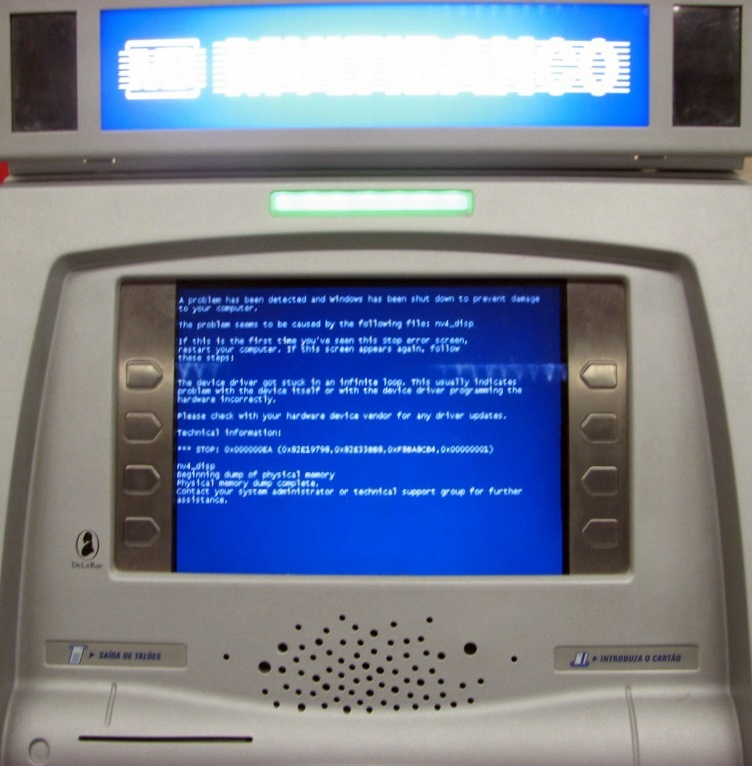
\includegraphics[width=.35\textwidth]{images/DeLaRue_ATM_Crash.jpg}
\end{center}

It turns out that most Windows crashes these days are caused not by
the Windows kernel itself, which is fairly bombproof, but instead by
Windows drivers, which run at the same protection level as the kernel. Scientists at Microsoft Research have integrated existing techniques
and new techniques to verify drivers. The Windows Driver Kit includes
the Static Driver Verifier\footnote{For more information, see
  \url{http://msdn.microsoft.com/en-us/windows/hardware/gg487506}.},
and any ``Certified for Windows'' product needs to pass the SDV.

Formal methods tools \emph{exhaustively} explore all possible states
of the system and driver. In particular, the SDV knows about all of the 
ways that the operating system can call the driver, and (symbolically) tries out
all of the combinations of calls that can occur.


\paragraph{Discussion.} In general, formal methods tools take a long time to run. Experts need to give hints to the tools so that they run in some reasonable amount of time.

Besides having to wait too long to get a result, and not being able to
get the verification to go through, the main shortcoming with formal
verification is that you can get (way too many) false positives: the
verification warns you of a problem that can never happen. This occurs
when the model is too coarse and includes cases that can never happen
in practice.

Formal methods are particularly useful when the problem domain is too
hard to reason about manually. Concurrency is a good example of such a 
domain.

\section*{Software Maintenance}
Your engineering programme has a lot of emphasis on design; who ever
heard of a Fourth Year Maintenance Project, for instance? Normally you start with a ``green field'': no code at all (or you're given some code and libraries but you start from close to nothing). When you go out on a co-op work term, chances are you'll be working on a project that is already well underway and possibly in the hands of customers (users). In the real world, maintenance accounts for a lot of engineer effort. In fact, in some long-running popular pieces of software, maintenance might be the majority of time spent.

\emph{Software maintenance} modifies existing software to fix defects,
improve performance, or make the software work in new environments
(porting)... after the software has shipped.

Software maintenance is hard. You have to understand the existing code,
which can be difficult (no matter whether you or someone else originally
wrote it). It's unglamorous, especially if you're fixing bugs. It's 
constrained; you better not break compatibility.

It is always tempting to start over from scratch; sometimes it looks
like the existing software is beyond hope, and it's more fun to redesign
rather than maintain.

\subsection*{Another Story from Ancient History (or: Motivation)}
\begin{quote}
	\emph{It's harder to read code than to write it.}
\end{quote}
	\hfill Joel Spolsky
	
Our lesson in history comes from \cite{spolsky:drw}.

Back in about the year 2000, Netscape (does anyone actually remember Netscape Navigator? It was a forerunner of Mozilla Firefox) decided that they were going to rewrite their browser code from scratch. This was widely considered a huge mistake -- it took them three years and in the meantime their old browser was out of date (and Microsoft Internet Explorer ended up taking a huge amount of market share, which was widely considered a disaster for internet standards). Netscape was by no means the only company to do this, but they were well known and make a good example.

Programmers are likely to say (and don't tell me you haven't said this when looking at some code): this code is a mess! It's got functions that are two pages long and it has 14 if-statements and calls a whole bunch of functions. Plus it's old, and newer is better, right?

Code doesn't degrade as it gets older. Unlike buildings, where the concrete crumbles and the steel rusts, new bugs don't appear magically in the software as time goes on. Code that is old is actually better, in some ways. It's been tested. Bugs have been fixed in it.

A long function that has 14 if-statements and all kinds of weird stuff in it? Those oddities are bug fixes. Maybe it's to handle a situation where the user is running with less than 1 GB of RAM; another handles the situation where the default temporary directory is not writeable; yet another makes no sense except it helps users who are still, for reasons nobody can explain, running Windows 98. Each of those bugs was discovered after testing and it may have taken a lot of effort to uncover and fix.

Maybe the code has serious architectural problems, but those can be fixed by refactoring. Is the code slow and inefficient? This can also be fixed without throwing all the code away (take the class ``Programming for Performance'' if this is interesting to you). Is the code ugly with horrible names and inconsistent formatting? Yep, once again, refactoring. The best part is that refactoring, no matter how much you do, will be faster than rewriting it from the ground up.

When you start from scratch, you are throwing away a lot of collected knowledge and bug fixes.

In fact, the \emph{second system effect} says that you may well do worse by starting over. Small, successful systems tend to have very complicated successors. The second system effect is also sometimes explained as ``Generals are always trying to fight the last war.'' When designing the new system, it's frequently the case that developers are trying to include all the things they wish had been in the first system. They might also lose track of what made the first system successful.



\subsection*{Types of Maintenance}
It turns out that a lot of software maintenance goes beyond
fixing bugs. According to T.~M. Pigosky~\cite{pswm},
approximately 80\% of software maintenance activities are unrelated to
defect fixes.  Here's a classification of different types of
maintenance; these all apply to already-shipped code.
\begin{itemize}
\item \emph{Corrective Maintenance}: correct known defects;
\item \emph{Adaptive Maintenance}: keep a software product usable in a changing environment;
\item \emph{Perfective Maintenance}: improve performance or maintainability; and
\item \emph{Preventive Maintenance}: correct latent faults in the product before they manifest themselves.
\end{itemize}

Some examples of each of the different kinds follow below.

When doing Corrective Maintenance, you remove a bug that is known to exist. You come across a piece of code that reads \texttt{getAppliance().activate(item);} and this results in a \texttt{NullPointerException} if \texttt{item} is \texttt{null}. Corrected by adding a null-check around that statement, such as:
\begin{verbatim} 
if (item != null) {
     getAppliance().activate(item);
}
\end{verbatim}

An example of Adaptive Maintenance would be changing your software product to conform to new security and data storage guidelines when Android 5.0 is released. It might also be that there's a new version of the user interface guidelines made available and you want your application to use the new format. This is sometimes optional (generally operating systems don't force the upgrade immediately and maintain backwards-compatibility for a number of years), but other times it is necessary: perhaps the government will no longer accept tax declarations via http and will accept them only via https (secure) starting from 1 January next year and if the changes are not made then on 1 January the system will simply stop working.

Perfective Maintenance can certainly include refactoring (see earlier lectures on that subject), but it is not limited to that. As a performance example, you might query some records from the database and then sort them in-memory in the program. This is inefficient; it would be better to rewrite this so the database records are returned already sorted. 

Preventive Maintenance is not very common, but sometimes in working on a software product a developer discovers a problem which will occur in the future. One of the most famous examples was the ``Y2K'' bug; in old computer systems which used two digits to represent the year, it was always assumed that the year was 1900 + the two digit year (so ``85's' represented 1985). The year 2000 would then be erroneously represented as 1900. To prevent this, many systems needed to be changed to 4-digit dates.


The lines between the different categories are not necessarily clearly defined. Users love to report bugs that are really new feature requests. Sometimes when you look at something, it's obviously a bug: there is a crash, the program throws a \texttt{NullPointerException}, or user data isn't saved when a user clicks the save button. 

Your users don't usually care about any line of distinction between a bug or feature: if they want to do something and the software does not support it (whether it's due to function not implemented or that function having a bug), the cause is irrelevant; all they care about out is that they can't accomplish whatever they wanted to do \cite{atwood:bfr}.

Sometimes, whether something is classified as a bug or new feature has some planning or financial consequences. It's possible to charge your customers for a features, but they're unlikely to pay for bug fixes. Also, bug fixes will likely be ported to earlier, already-released versions of the software, while new features will have to wait for the next release. How exactly a ticket is classified will vary depending on your project's rules.

Patching can be problematic and lead to gnarly code with no
design. What's the solution? Managing maintenance.

\paragraph{Managing Maintenance.}
Software projects are huge and therefore have huge numbers of defects,
shipped software is by no means exempt from defects. Many projects
have tens of thousands of known defects The average bug lifetime in the Linux kernel was once measured at 1.38 years. Years!

Triage is key to avoiding analysis paralysis: some defects are more
important than others. Security fixes should go in right away, while
minor defects can wait. For instance, Microsoft has deployed monthly
software patches in the past (``patch Tuesday''), but pushes security fixes as needed.

When you have multiple concurrent branches of the software, it will be necessary to make decisions about how to proceed with patches. As the branches diverge, it becomes harder and harder to move changes from one branch to another. At some point, moving a bug fix into a previous version is not worth the effort.

For sufficiently large projects, there might be a person charged with managing maintenance: the release manager. A release manager must be knowledgeable about software engineering in general, but takes responsibility for: assembling all the various updates, deciding when to make a new release, and troubleshoot problems caused by an update~\cite{relman}.

\paragraph{Patch Discipline.} Any change can cause problems, even
more problems than it solves. Before pushing a change, be sure to
check that it makes things better rather than worse. Testing is
particularly critical; imagine what would happen if a patch to the
Microsoft Windows operating system caused 1\% of the world's computers
to break down?

You can use reviews, regression tests, and other verification
techniques to help ensure that you do less harm than good.

\paragraph{Agreements.}
It does not happen much for consumers, but when large organizations buy (or license) some software, they often want to have a signed maintenance agreement. In such a contract, both parties need to agree on the answers to these important questions~\cite{outlaw}:

\begin{enumerate}
	\item What constitutes a defect in the software?
	\item What types of defect, if any, are not covered?
	\item How to categorize a defect (priority 1, 2, etc)?
	\item Who is responsible for categorization?
	\item What is the flexibility of categories/ ability to escalate?
	\item What are the response times and resolution times promised?
	\item What are the support hours, and what are the overtime charges, if any?
	\item Will the supplier be expected to travel to the customer to fix defects?
	\item Are new releases included or just patches?
	\item Will old versions cease to be supported at some point?
	\item Can the customer delay installation of a patch?
	\item How regularly are upgrades to be provided?
	\item How are charges and payment settled?
\end{enumerate}

Plus some of the usual contract items such as renewal, applicability, jurisdiction, et cetera. For full details on contract law, consult a lawyer.

\paragraph{Retirement.}
Eventually it might be time to retire a piece of software -- to officially end its development and support. This is often a business decision: sales or support contracts for something may no longer justify the cost and effort of maintaining it any longer. Where a successor product exists, a final maintenance project might be to add a utility to export the data from the old to the new product.


\bibliographystyle{alpha}
\bibliography{155}


\end{document}
